\section{Ergebnisse} % (fold)
    \label{sec:ergebnisse}
    Im Folgenden werden die Ergebnisse der \NumWord{\theexperiment} ab \autopageref{exp:uniref90} beschriebenen Experimente dargestellt. Der Hauptfokus liegt dabei auf der Datenbankgröße und Erkennungsperformanz. Ein Abschnitt zur Reproduzierbarkeit ist in \Anhang{README.txt} vermerkt.

    \subsection{UniRef90 Sampling} % (fold)
        \label{sub:uniref90_results}

        Beim UniRef90 Sampling wurden die Amplituden-Grenzwerte für vier verschiedene Signifikanzniveaus ermittelt, für 5\%, 0.1\%, 0.01\% und 0.001\%, um dadurch die Frequenzen mit den als Ausreißer definierten Amplituden als signifikant zu identifizieren. In \MyRef{fig:frequencies_normal} ist die Auswahlhäufigkeit der Frequenzen in der bisherigen Implementierung von \protfin\ dargestellt, bevor die ermittelten Grenzwerte einbezogen wurden.

        \begin{figure}[H]
            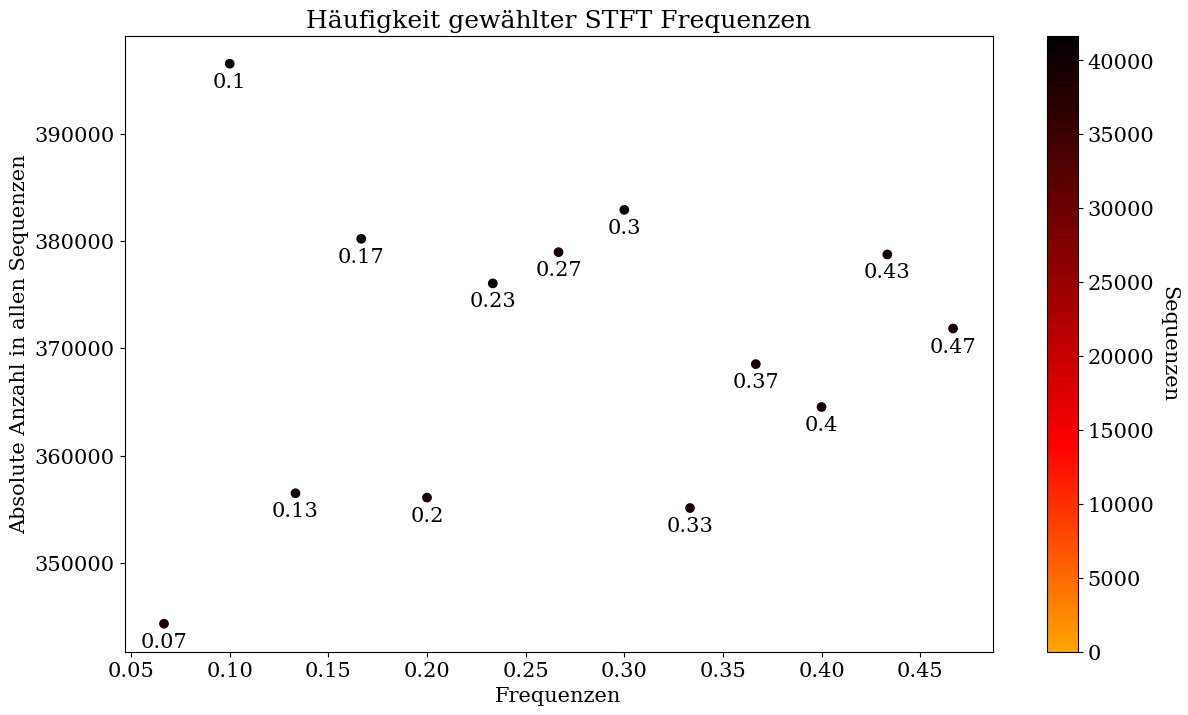
\includegraphics[width=\textwidth]{frequencies_normal.png}
            \caption[Häufigkeit gewählter Frequenzen über alle \aclp{TP} vor \Exp{exp:uniref90}]{Häufigkeit gewählter Frequenzen über alle \acp{TP} vor \Exp{exp:uniref90}: Die Häufigkeiten, wie oft eine Frequenz in einer Sequenz gewählt wird, werden über alle \acp{TP} summiert (y-Achse). Die Bezeichnungen an den Punkten repräsentieren die genaue Frequenz, wie auf der x-Achse dargestellt. Das Reziproke einer Frequenz bedeutet die Länge der Periode. Die Farbe der Punkte gibt an, in wie vielen Sequenzen die jeweilige Frequenz vorkam. Die Werte wurden expemplarisch für \acl{FG} 30 mit Überlappung 15 und $n\_peaks=alle$ (siehe \MyRef{sub:durchfuhrung}) durchgeführt, allerdings nur für den \ac{KF} Hydrophobizität.}
            \label{fig:frequencies_normal}
        \end{figure}

        Die Häufigkeiten der Frequenzen lagen bisher in \protfin\ im Mittel bei ungefähr 360000, was bei circa 40000 Proteinen bedeutet, dass in einer Aminosäuresequenz jede Frequenz etwa 9-mal vorkommt. Frequenz 0.1, also eine Periode von jeder 10. Aminosäure (das Reziproke der Frequenz ist die Länge der Periode), scheint zudem besonders häufig gewählt zu werden.

        \begin{figure}[H]
            \centering
            \begin{subfigure}{.45\textwidth}
                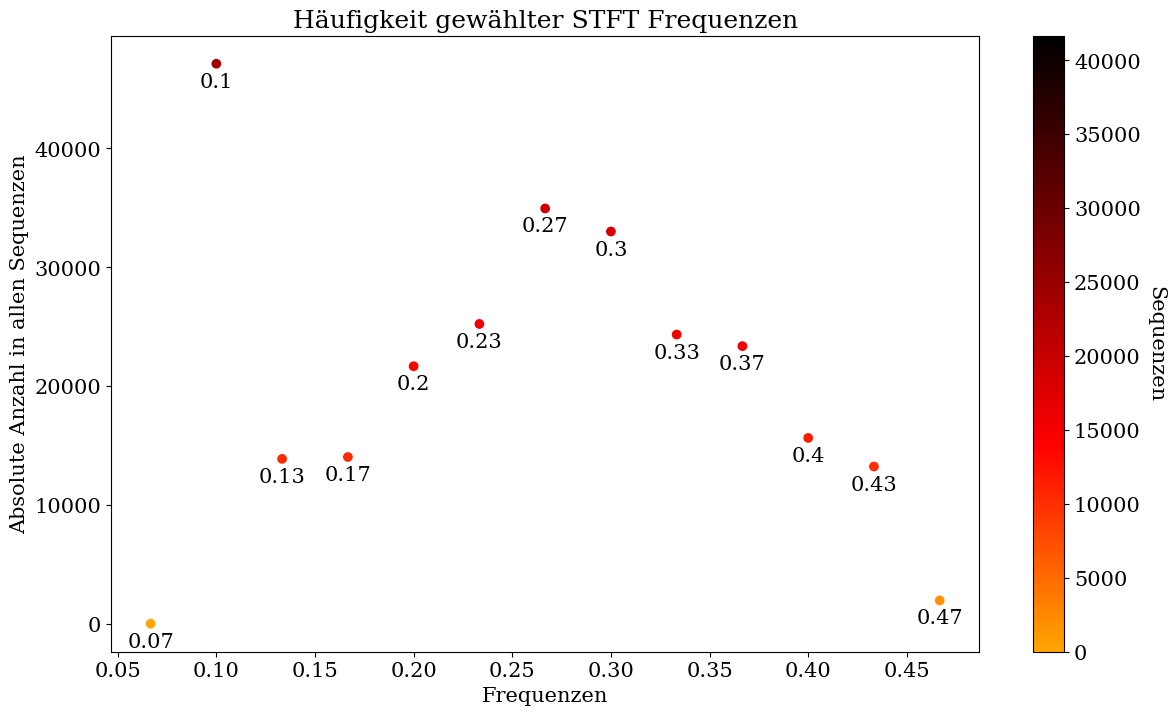
\includegraphics[width=\textwidth]{frequencies_5.png}
                \caption{$\alpha=5\%$}
                \label{fig:frequencies_5}
            \end{subfigure}
            \begin{subfigure}{.45\textwidth}
                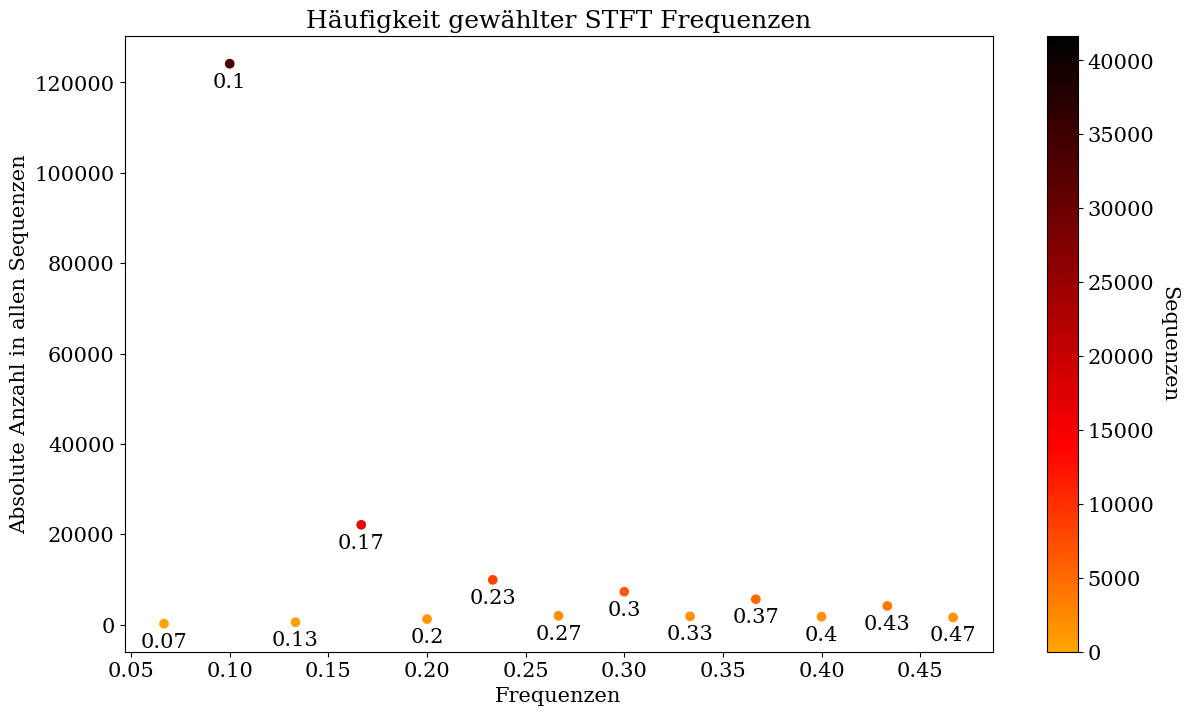
\includegraphics[width=\textwidth]{frequencies_0.1.png}
                \caption{$\alpha=0.1\%$}
                \label{fig:frequencies_0.1}
            \end{subfigure}\\
            \begin{subfigure}{.45\textwidth}
                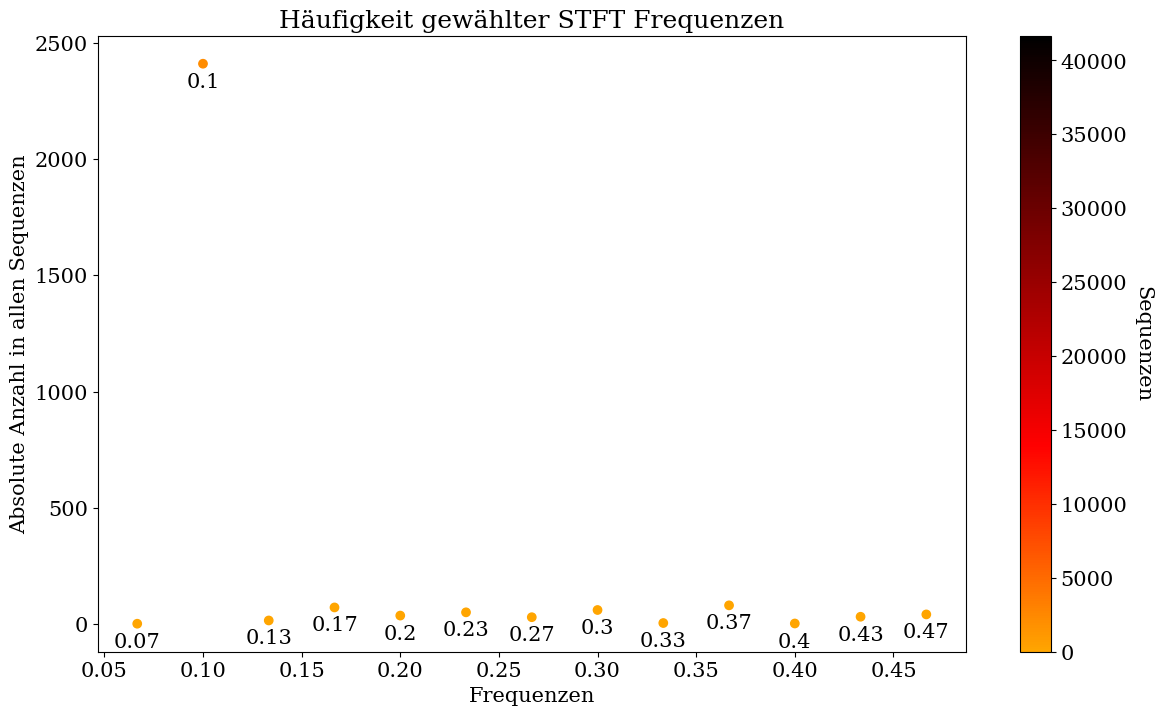
\includegraphics[width=\textwidth]{frequencies_0.01.png}
                \caption{$\alpha=0.01\%$}
                \label{fig:frequencies_0.01}
            \end{subfigure}
            \begin{subfigure}{.45\textwidth}
                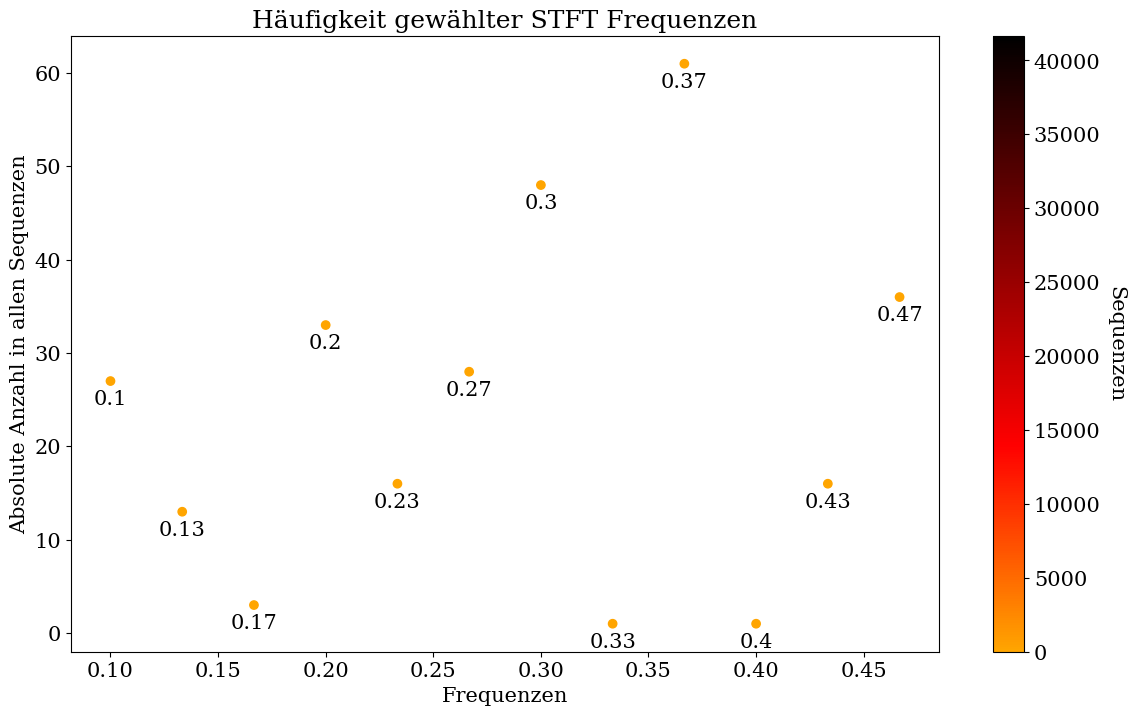
\includegraphics[width=\textwidth]{frequencies_0.001.png}
                \caption{$\alpha=0.001\%$}
                \label{fig:frequencies_0.001}
            \end{subfigure}
            \caption[Häufigkeit gewählter Frequenzen über alle \aclp{TP} nach \Exp{exp:uniref90}]{Häufigkeit gewählter Frequenzen über alle \acp{TP} nach \Exp{exp:uniref90}: Die Häufigkeiten, wie oft eine Frequenz in einer Sequenz gewählt wird, werden über alle \acp{TP} summiert (y-Achse). Die Bezeichnungen an den Punkten repräsentieren die genaue Frequenz, wie auf der x-Achse dargestellt. Das Reziproke einer Frequenz bedeutet die Länge der Periode. Die Farbe der Punkte gibt an, in wie vielen Sequenzen die jeweilige Frequenz vorkam. Die Werte wurden expemplarisch für \acl{FG} 30 mit Überlappung 15 und $n\_peaks=alle$ (siehe \MyRef{sub:durchfuhrung}) durchgeführt. Die Signifikanzniveaus bedeuten, dass $\alpha$ und $1-\alpha$ als Grenzwert für die Selektion verwendet wurden.}
            \label{fig:frequencies_uniref}
        \end{figure}

        \MyRef{fig:frequencies_uniref} zeigt, wie häufig die einzelnen Frequenzen nach Einbezug der Grenzwerte ausgewählt wurden. Wie \MyRef{fig:frequencies_normal} ist die Selektion nur exemplarisch für \ac{FG} 30 mit Überlappung von 15 und $n\_peaks = alle$, hier allerdings mit Beachtung aller \acp{KF}. Es wurden nicht mehr Parameter dargestellt, weil primäres Ziel die Ermittlung der Grenzwerte je Signifikanzniveau war, \MyRef{exp:target_zone} wurde mit derselben Selektionsmethode für alle Parameter mit $\alpha=5\%$ durchgeführt. Die Ergebnisse dazu sind ab \autopageref{sub:target_results} zu finden. Für \MyRef{exp:selection_method} wurden alle Signifikanzniveaus verwendet, allerdings mit anderen Selektionsansätzen.

        Die Häufigkeiten werden mit schrumpfendem $\alpha$ deutlich kleiner. So kommt eine Frequenz mit 5\% Grenze im Mittel nur in etwa jeder zweiten Sequenz vor, und ab 0.1\% noch deutlich seltener. Die maximalen Häufigkeiten liegen bei unter 200, wobei auch die Anzahl verschiedener Frequenzen sinkt. So sind es in \MyRef{fig:frequencies_0.001} nur sechs verschiedene, mit einer maximalen Auswahlrate von etwa 40 Mal. Im Vergleich zu \MyRef{fig:frequencies_normal} mit nur einem betrachteten \ac{KF} gab es eine sehr starke Reduktion in der Auswahl.

        Ursprünglich war \MyRef{exp:uniref90} so konzipiert, dass nur ein 5\%-alpha ermittelt wird. Da die Datenbanken aber weiterhin zu groß waren, wie in \MyRef{fig:uniref90.sp}, \MyRef{sub:filter_results} und \MyRef{sub:target_results} zu sehen, wurde es um die strengeren Signifikanzniveaus erweitert. Die Identifizierung ist ab \ac{FG} 20 sehr gut und hat eine nahezu 100\%-ige Schärfe. \ac{FG} 10 ist zwar unter der Eingabegröße der Datenbank, scheitert aber bei der Identifikation (Unique Self Matches) und wurde daher nicht für alle Experimente betrachtet. 

        \begin{figure}[H]
            \centering
            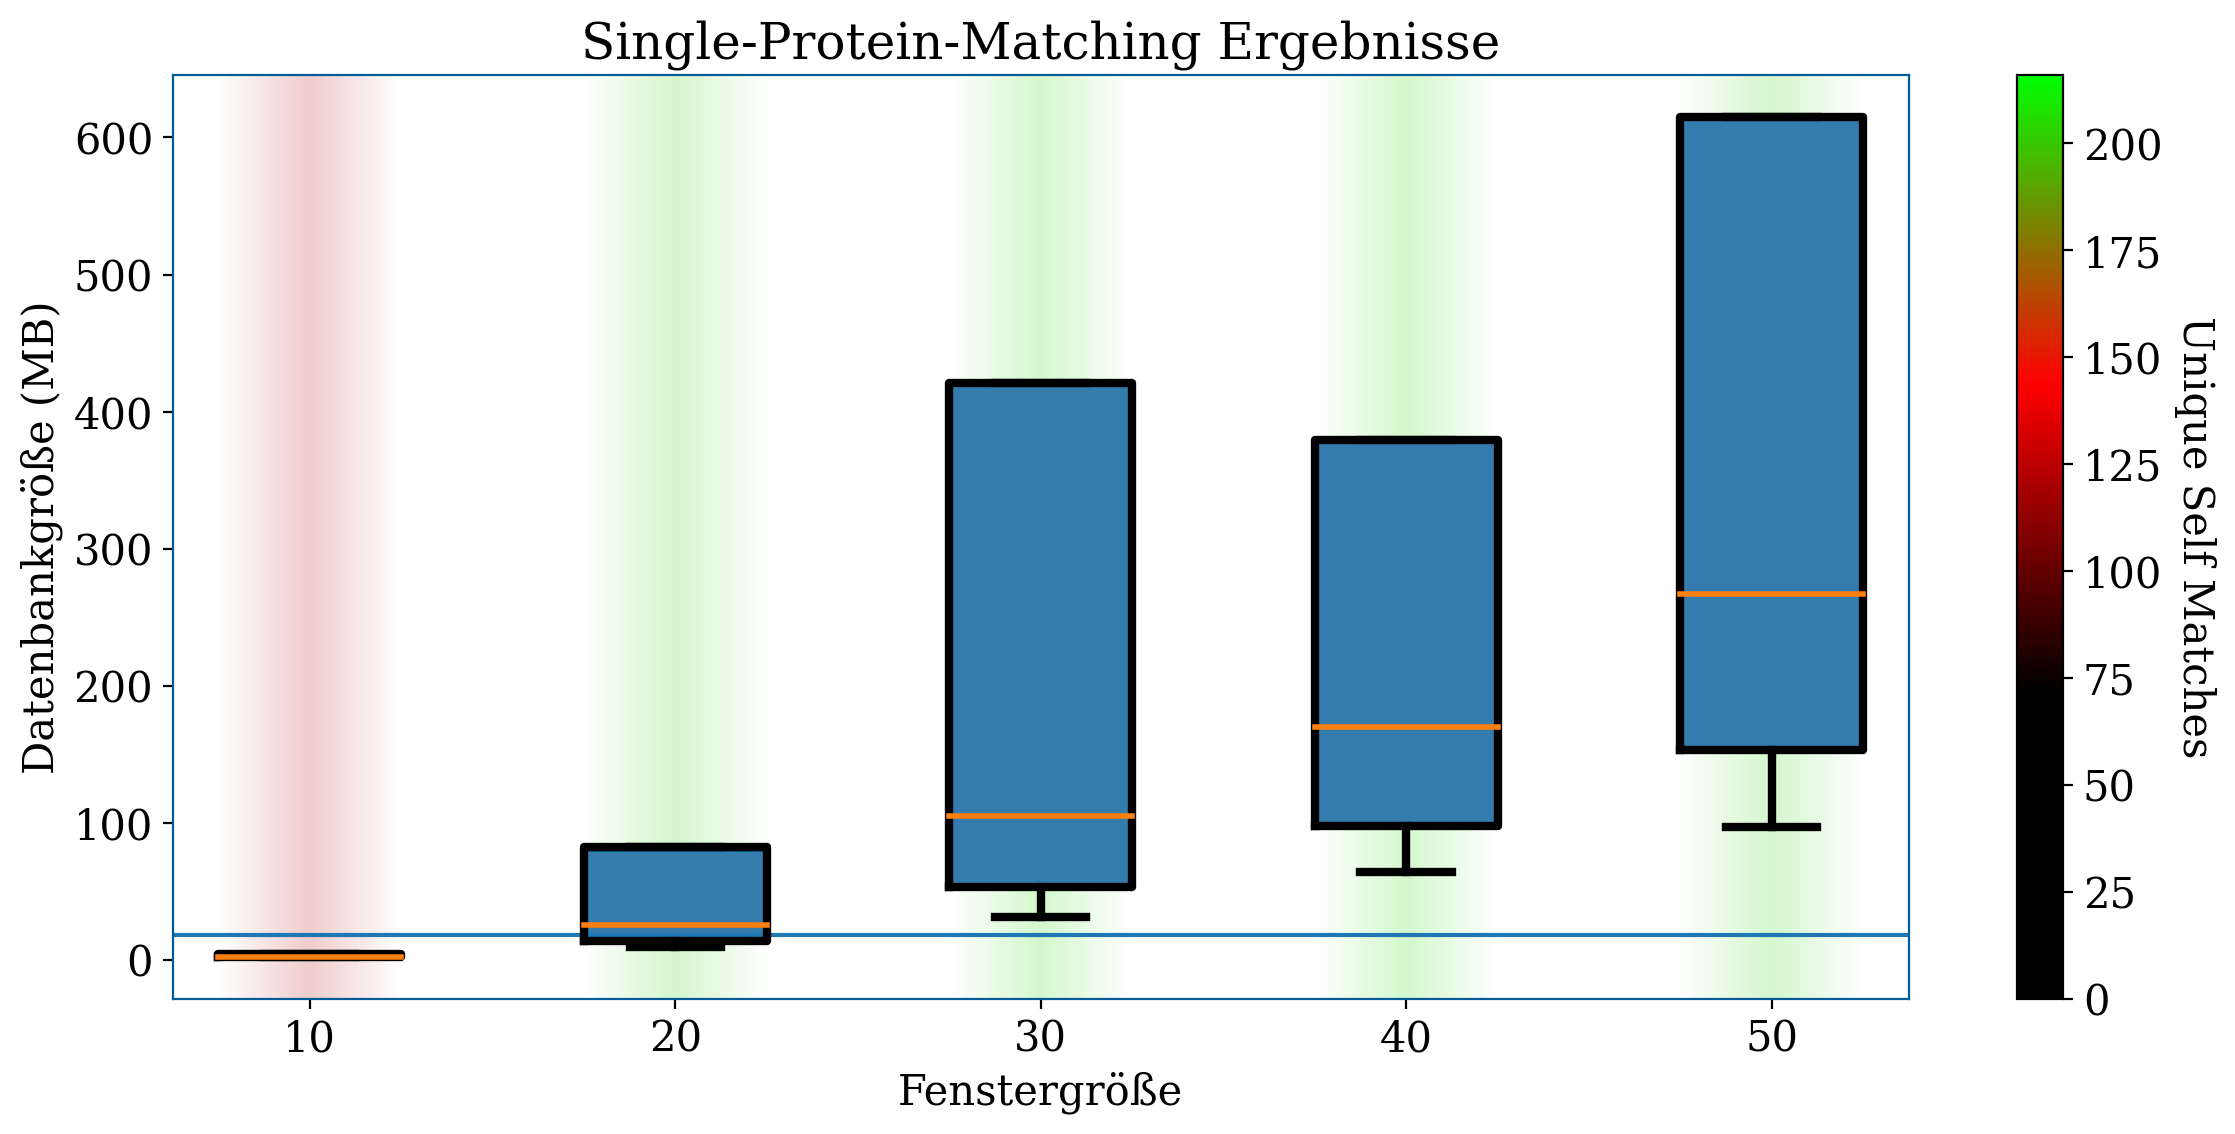
\includegraphics[width=\textwidth]{plot_uniref90.sp.png}
            \caption[Single-Protein-Matching \Exp{exp:uniref90}]{Single-Protein-Matching-Ergebnisse für $\alpha=5\%$: Die Boxen bilden die Datenbankgrößen für die verschiedenen Parameter aus \MyRef{tab:parameter} ab. Die blaue Füllung repräsentiert die Schärfe (\MyRef{equ:f_score}), sofern sie einen positiven Wert hat. Je mehr die Box also prozentual gefüllt ist, desto höher ist die Schärfe (bei Schärfe 0.5 wäre sie halb voll). Die farbige Fläche über und unter den Boxen stellt die Anzahl dar, wie viele der Suchproteine als Treffer mit alleinigem besten Score identifiziert wurden (hier ``Unique Self Matches''). Die blaue horizontale Linie kennzeichnet die Größe der Eingabedaten. Die genauen Werte dieses Plots sind in den Dateien \Anhang{UniRef90 Sampling/*} zu finden.}
            \label{fig:uniref90.sp}
        \end{figure}
    % subsection uniref90_sampling (end)
    \subsection{Filter Hashes} % (fold)
        \label{sub:filter_results}
        In \MyRef{exp:filter_hashes} war die Intention, in vielen Proteinen auftretende Hashes aus der Datenbank herauszufiltern, da Hashes, die in nahezu allen Proteinen vorkommen, bei der Identifikation eines Proteins wenig Bedeutung haben sollten. Bei der Durchführung der Experimente wurden die seltenen Hashes nach Quantil behalten. Getestet werden sollten alle Quantile in 10\%-Schritten von 10\% bis 100\%, Letzteres als Nullprobe ohne Filtern. Aufgrund eines Eingabefehlers wurde der geplante Parameter $Quantil=0.8$ ausgelassen (\protfin\ wurde ``\texttt{.8.}'' übergeben statt ``\texttt{.8}'' und konnte den Wert nicht als \texttt{float} parsen).

        Es wurden beide Matching-Ansätze durchgeführt (siehe ab \autopageref{sp.matching}). Die Ergebnisse für das Single-Protein-Matching sind in \MyRef{fig:filter_hashes.sp} dargestellt.

        \begin{figure}[H]
            \centering
            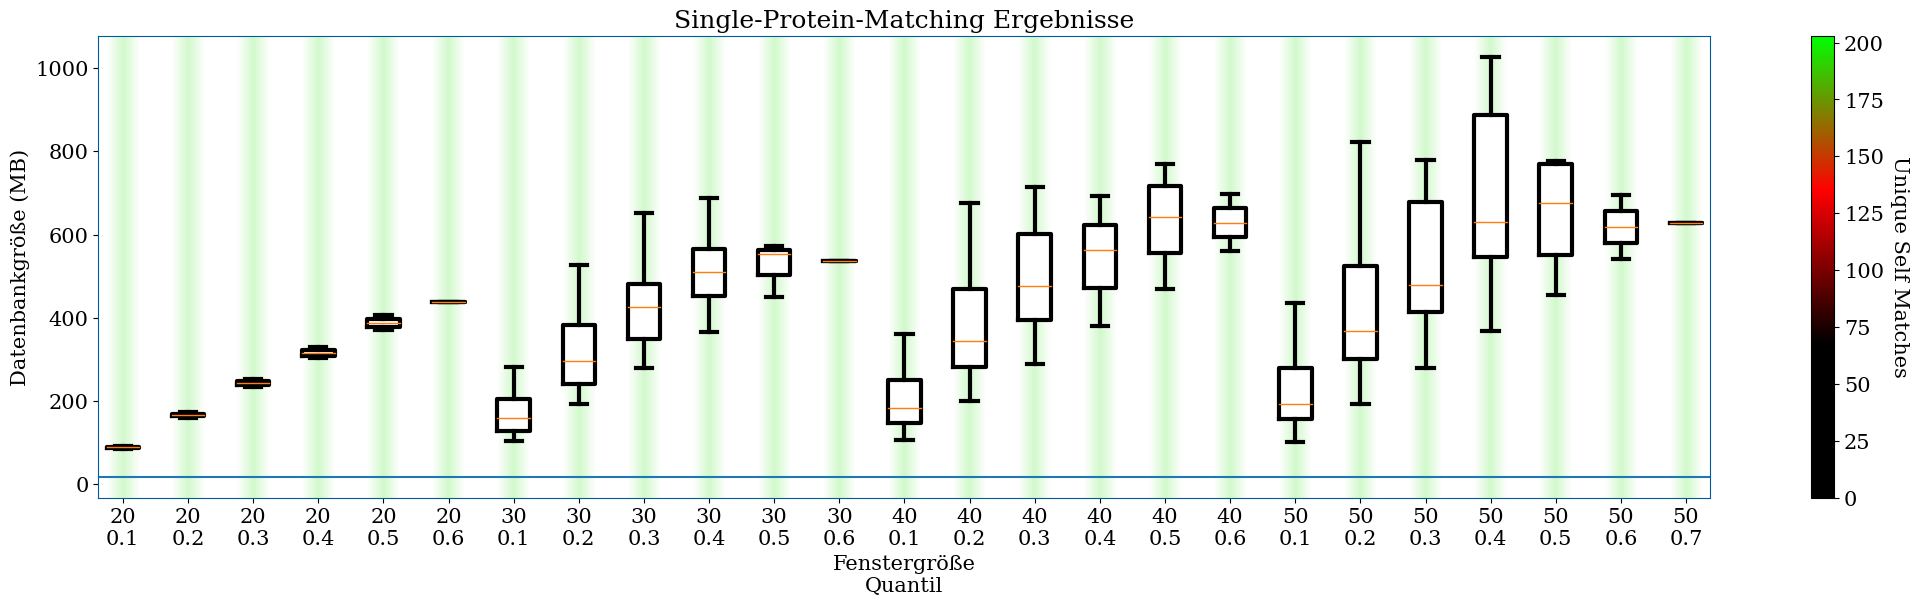
\includegraphics[width=\textwidth]{plot_filter_hashes.sp.png}
            \caption[Single-Protein-Matching \Exp{exp:filter_hashes}]{Single-Protein-Matching-Ergebnisse: Die Boxen bilden die Datenbankgrößen für die verschiedenen Parameter aus \MyRef{tab:parameter} ab, wobei das Experiment aufgrund zu hoher Laufzeit für die oberen Filterquantile vorzeitig abgebrochen wurde. Die blaue Füllung repräsentiert die Schärfe (\MyRef{equ:f_score}), sofern sie einen positiven Wert hat. Das heißt, je mehr die Box prozentual gefüllt ist, desto höher ist die Schärfe (bei Schärfe 0.5 wäre sie halb voll). Die farbige Fläche über und unter den Boxen stellt die Anzahl dar, wie viele der Suchproteine als Treffer mit alleinigem besten Score identifiziert wurden (hier ``Unique Self Matches''). Die blaue horizontale Linie kennzeichnet die Größe der Eingabedaten. Die Originaldaten für diesen Plot sind in den Dateien \Anhang{Filter Hashes/*} zu finden.}
            \label{fig:filter_hashes.sp}
        \end{figure}

        Aufgrund zu langer Laufzeit wurde das Single-Protein-Matching vorzeitig abbgebrochen, sodass die Daten der pro \ac{FG} jeweils letzten Quantile nicht vollständig sind. \MyRef{fig:filter_hashes.sp} zeigt für die Suchproteine für alle getesteten Parameter eine hohe Identifikationsrate mit hoher Schärfe. Mit sinkendem Quantil schrumpft auch die Datenbankgröße annähernd linear. Dennoch ist keine davon unter dem Limit der Eingabe.

        Der Family-Matching-Ansatz in \MyRef{fig:filter_hashes.fam} hat eine geringe Schärfe von unter 0.5, wobei sich für die getesteten Parameter zeigt, dass kleinere Quantile einen höheren F1-Score haben, der aber deutlich unter 1 liegt. Zwischen dem 70\%- und 100\%-Quantil deutet sich ein leichter Anstieg des F1-Scores an.

        \begin{figure}[H]
            \centering
            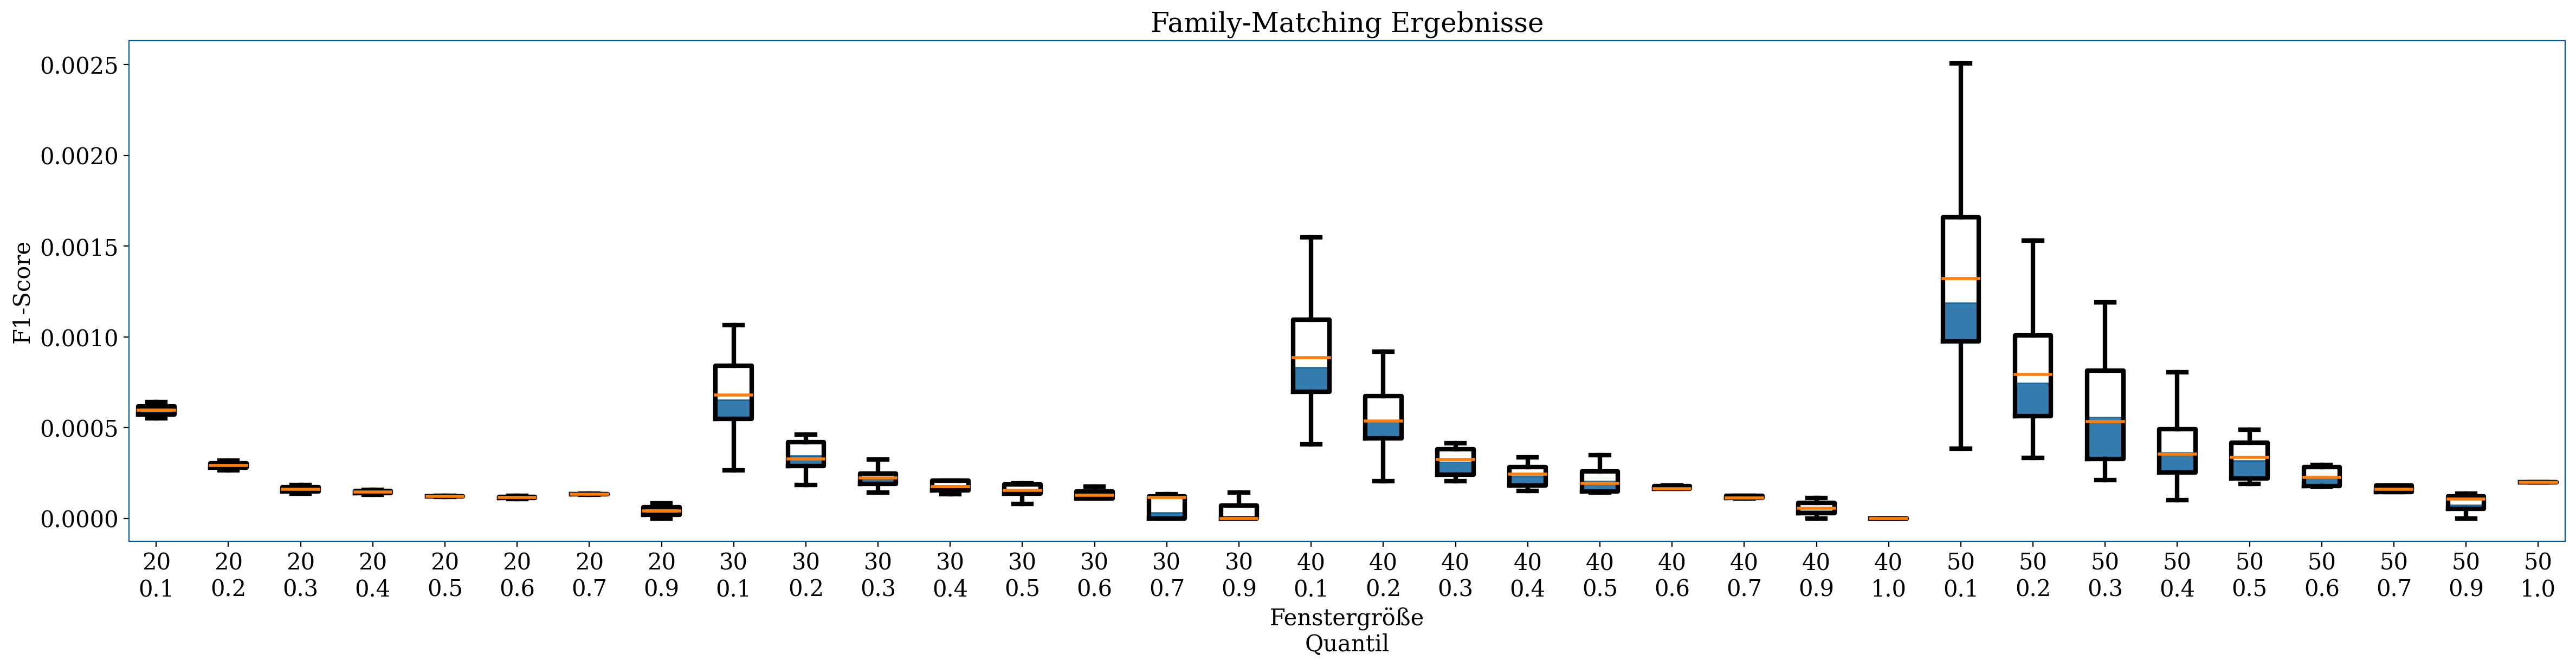
\includegraphics[width=\textwidth]{plot_filter_hashes.fam.png}
            \caption[Family-Matching \Exp{exp:filter_hashes}]{Family-Matching-Ergebnisse: Die Boxen bilden die mittleren F1-Scores (siehe \MyRef{equ:f_score}) für die verschiedenen Parameter aus \MyRef{tab:parameter} ab. Die blaue Füllung repräsentiert die Schärfe (\MyRef{equ:f_score}), sofern sie einen positiven Wert hat. Das heißt, je mehr die Box prozentual gefüllt ist, desto höher ist die Schärfe (bei Schärfe 0.5 wäre sie halb voll). Die exakten Werte der Ergebnisse, die abgebildet sind, sind in \Anhang{Filter Hashes/summary\_match\_family.csv} abgelegt.}
            \label{fig:filter_hashes.fam}
        \end{figure}

    \subsection{Target-Zone} % (fold)
        \label{sub:target_results}
        In \MyRef{exp:target_zone} wurde der Selektionsansatz aus \MyRef{exp:uniref90} mit $\alpha=5\%$ verwendet, was somit eine Erweiterung der Ergebnisse aus \MyRef{sub:uniref90_results} darstellt. Wie dort wird hier lediglich der Single-Protein-Matching-Ansatz durchgeführt, allerdings mit dem Unterschied, dass die in \MyRef{exp:target_zone} beschriebene \acl{TZ} eingeschränkt wird. Getestet werden die Werte 8, 16, 32, 64, da sich diese Werte auf eine ganze Zahl an Bits aufteilen lassen (3, 4, 5, 6), um in den Hash (\MyRef{fig:hash}) einzufließen.

        Für das Testen verschiedener \acp{TZ} ist in \MyRef{fig:target_zone.sp} eine Tendenz zu exponentiellem Wachstum der Datenbankgröße bei ansteigender \ac{TZ} erkennbar. Je kleiner die \acl{FG} und je kleiner die \ac{TZ}, desto kleiner wird die Datenbank. Wie beim Sampling in \MyRef{fig:uniref90.sp} scheitert die Identifikation bei \ac{FG} 10 hinsichtlich der Unique Self Matches, im Gegensatz zu den anderen Größen, welche auch eine hohe Schärfe haben.

        \begin{figure}[H]
            \centering
            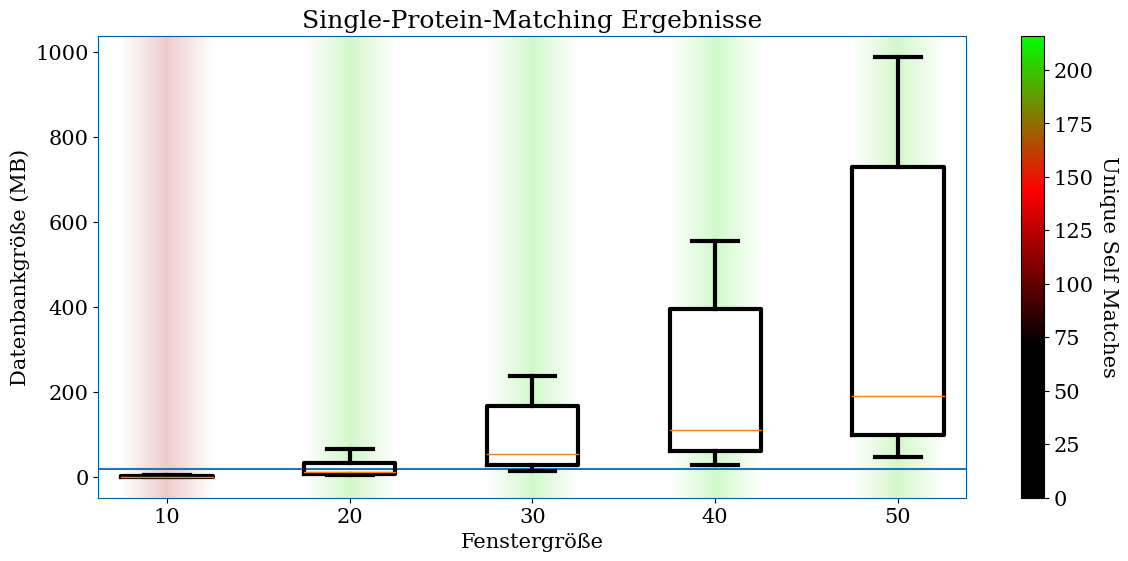
\includegraphics[width=\textwidth]{plot_target_zone.sp.png}
            \caption[Single-Protein-Matching \Exp{exp:target_zone}]{Single-Protein-Matching-Ergebnisse: Die Boxen bilden die Datenbankgrößen für die verschiedenen Parameter aus \MyRef{tab:parameter} ab. Die blaue Füllung repräsentiert die Schärfe (\MyRef{equ:f_score}), sofern sie einen positiven Wert hat. Das heißt, je mehr die Box prozentual gefüllt ist, desto höher ist die Schärfe (bei Schärfe 0.5 wäre sie halb voll). Die farbige Fläche über und unter den Boxen stellt die Anzahl dar, wie viele der Suchproteine als Treffer mit alleinigem besten Score identifiziert wurden (hier ``Unique Self Matches''). Die blaue horizontale Linie kennzeichnet die Größe der Eingabedaten. Die Werte für diesen Plot sind in den Dateien \Anhang{Target-Zone/*} zu finden.}
            \label{fig:target_zone.sp}
        \end{figure}

    \subsection{Selection-Method} % (fold)
        \label{sub:selection_results}
        Da das \MyRef{exp:target_zone} in \MyRef{sub:target_results} aufgrund zu hoher Laufzeit vorzeitig abgebrochen wurde, gibt es im Folgenden für eniige Paramter keine Ergebnisse. Es wurden beide Matching-Varianten (beschrieben auf \autopageref{sp.matching}) für die in \MyRef{tab:parameter} angegebenen Parameter durchgeführt und dabei drei verschiedene Ansätze der Selektion verfolgt.

        \subsubsection{Ansatz 1: Wahl der Frequenzen nur über Grenzwerte} % (fold)
            \label{ssub:ansatz_1_results}
            Der erste Ansatz verwendet die durch das Signifikanzniveau $\alpha$ definierten Randbereiche. Es werden nur die Frequenzen ausgewählt, deren Amplituden durch die Grenzwerte zu Ausreißern werden. In \MyRef{fig:selection_method.none.sp} sind die Ergebnisse des Single-Protein-Matchings abbgebildet. Für $\alpha=5\%$ gibt es keine Werte, weil die Datenbanken zu groß waren. Ebenfalls zu groß waren sie für alle $k=0$ und bei $\alpha=0.1$ zusätzlich bei $k=1$. Die besten Ergebnisse erzielen jedes Mal die Kombination aus $\alpha=0.001\%$ mit $k \in \{2, 3\}$, wo die Datenbanken auf Höhe der Eingabegröße liegen und alle Proteine eindeutig erkannt wurden. Die Schärfe liegt zudem jedes Mal bei nahezu 100\%.

            \begin{figure}[H]
                \includegraphics[width=\textwidth]{plot_selection_method_none.sp.png}
                \caption[Single-Protein-Matching \Exp{exp:selection_method}, Ansatz 1: Wahl nur mit Grenzwerten]{Single-Protein-Matching \Exp{exp:selection_method}, Ansatz 1: Wahl nur mit Grenzwerten: Die Boxen bilden die Datenbankgrößen für die verschiedenen Parameter aus \MyRef{tab:parameter} ab. Die blaue Füllung repräsentiert die Schärfe (\MyRef{equ:f_score}), sofern sie einen positiven Wert hat. Das heißt, je mehr die Box prozentual gefüllt ist, desto höher ist die Schärfe (bei Schärfe 0.5 wäre sie halb voll). Die farbige Fläche über und unter den Boxen stellt die Anzahl dar, wie viele der Suchproteine als Treffer mit alleinigem besten Score identifiziert wurden (hier ``Unique Self Matches''). Die blaue horizontale Linie kennzeichnet die Größe der Eingabedaten. Die Daten für die Abbildungen sind in den Dateien \Anhang{Selection-Method/*} abgelegt (Werte bei Spalte \texttt{Selection\_Method}$=$\texttt{none}).}
                \label{fig:selection_method.none.sp}
            \end{figure}

            Die Ergebnisse des Family-Matchings sind in \MyRef{fig:selection_method.none.fam} dargestellt. Wie auch beim Single-Protein-Matching in \MyRef{fig:selection_method.none.sp} ist die Performanz für die getesteten Signifikanzniveaus unter 5\% für $k \in \{2, 3\}$ immer die beste. Der höchste F1-Score von etwa $33\times 10^{-4}$ wird für \ac{FG} 50 mit 50\% Überlappung, $n\_peaks=3$ und $k=3$ erzielt. Die Schärfe liegt bei allen Werten unter 50\%.

            \begin{figure}[H]
                \includegraphics[width=\textwidth]{plot_selection_method_none.fam.png}
                \caption[Family-Matching \Exp{exp:selection_method}, Ansatz 1: Wahl nur mit Grenzwerten]{Family-Matching \Exp{exp:selection_method}, Ansatz 1: Wahl nur mit Grenzwerten: Die Boxen bilden die mittleren F1-Scores (siehe \MyRef{equ:f_score}) für die verschiedenen Parameter aus \MyRef{tab:parameter} ab. Die blaue Füllung repräsentiert die Schärfe (\MyRef{equ:f_score}), sofern sie einen positiven Wert hat. Das heißt, je mehr die Box prozentual gefüllt ist, desto höher ist die Schärfe (bei Schärfe 0.5 wäre sie halb voll). Die originalen Werte für diesen Plot sind in \Anhang{Selection-Method/summary\_match\_family.csv} zu finden (Werte bei Spalte \texttt{Selection\_Method}$=$\texttt{none}).}
                \label{fig:selection_method.none.fam}
            \end{figure}
        % subsubsection ansatz_1_wahl_der_frequenzen_nur_über_grenzwerte (end)

        \subsubsection{Ansatz 2: Wahl der Frequenzen über Ausreißer in den Extrempunkten} % (fold)
        \label{ssub:ansatz_2_results}
        Über den zweiten Ansatz der Frequenzwahl werden die Frequenzen in zwei Schritten selektiert. Zuerst werden diejenigen behalten, deren Amplituden ein lokales Extremum darstellen. Anschließend werden von diesen wiederum nur welche behalten, deren Amplituden durch das entsprechende Signifikanzniveau $\alpha$ als Ausreißer definiert werden. Demzufolge erweitert dieser Ansatz den Ersten (\MyRef{ssub:ansatz_1_results}) um die Vorselektion durch Extremwerte. Hierfür wurden beide Matching-Ansätze (beschrieben auf \autopageref{sp.matching}) für die in \MyRef{tab:parameter} angegebenen Parameter getestet. Die Single-Protein-Matching-Ergebnisse sind in \MyRef{fig:selection_method.absolute.sp} zusammengefasst.
        
        \begin{figure}[H]
            \includegraphics[width=\textwidth]{plot_selection_method_absolute.sp.png}
            \caption[Single-Protein-Matching \Exp{exp:selection_method}, Ansatz 2: Wahl der Ausreißer der lokalen Maxima/Minima]{Single-Protein-Matching \Exp{exp:selection_method}, Ansatz 2: Wahl der Ausreißer der lokalen Maxima/Minima: Die Boxen bilden die Datenbankgrößen für die verschiedenen Parameter aus \MyRef{tab:parameter} ab. Die blaue Füllung repräsentiert die Schärfe (\MyRef{equ:f_score}), sofern sie einen positiven Wert hat. Das heißt, je mehr die Box prozentual gefüllt ist, desto höher ist die Schärfe (bei Schärfe 0.5 wäre sie halb voll). Die farbige Fläche über und unter den Boxen stellt die Anzahl dar, wie viele der Suchproteine als Treffer mit alleinigem besten Score identifiziert wurden (hier ``Unique Self Matches''). Die blaue horizontale Linie kennzeichnet die Größe der Eingabedaten. Die Daten für die Abbildungen sind in den Dateien \Anhang{Selection-Method/*} abgelegt (Werte bei Spalte \texttt{Selection\_Method}$=$\texttt{absolute}).}
            \label{fig:selection_method.absolute.sp}
        \end{figure}

        Die Ergebnisse sind dem ersten Ansatz in \MyRef{fig:selection_method.none.sp} sehr ähnlich: Nicht vertreten ist $\alpha=5\%$, aufgrund zu großer Datenbanken. Die besten Werte erzielen $k \in \{2, 3\}$ für die restlichen Signifikanzniveaus, wobei das 0.1\%-Quantil für $k$ vertreten ist. Die Unterschiede liegen in einer geringeren Streuung der Datenbankgrößen und der Tatsache, dass $k=0$ Ergebnisse besitzt. Die Werte für $k \in \{0, 1\}$ sind dabei identisch, da Frequenz 0 als Randfrequenz nicht als Extremwert infrage kommt und bei $k=1$ folglich nicht entfernt werden kann. Es wurden jedes Mal alle Proteine mit einer nahezu 100\%-igen Schärfe wiedererkannt.

        Die Ergebnisse des Family-Matchings sind in der nachfolgenden \MyRef{fig:selection_method.absolute.fam} zu sehen und den Ergebnissen aus dem ersten Ansatz ebenfalls ähnlich (\MyRef{fig:selection_method.none.fam}): Die besten Werte erzielen $k \in \{2, 3\}$ für die restlichen Signifikanzniveaus, wobei $\alpha=0.1\%$ für $k$ vertreten ist, aber generell die Streuung der F1-Scores geringer ist. Der höchste F1-Score von etwa $33\times 10^{-4}$ wird hier ebenfalls für \ac{FG} 50 mit 50\% Überlappung und $n\_peaks=3$ erzielt, allerdings mit $k=2$. Bei allen Werten wird ebenfalls eine Schärfe von unter 0.5 erreicht.

        \begin{figure}[H]
            \includegraphics[width=\textwidth]{plot_selection_method_absolute.fam.png}
            \caption[Family-Matching \Exp{exp:selection_method}, Ansatz 2:  Wahl der Ausreißer der lokalen Maxima/Minima]{Family-Matching \Exp{exp:selection_method}, Ansatz 2:  Wahl der Ausreißer der lokalen Maxima/Minima: Die Boxen bilden die mittleren F1-Scores (siehe \MyRef{equ:f_score}) für die verschiedenen Parameter aus \MyRef{tab:parameter} ab. Die blaue Füllung repräsentiert die Schärfe (\MyRef{equ:f_score}), sofern sie einen positiven Wert hat. Das heißt, je mehr die Box prozentual gefüllt ist, desto höher ist die Schärfe (bei Schärfe 0.5 wäre sie halb voll). Die originalen Werte für diesen Plot sind in \Anhang{Selection-Method/summary\_match\_family.csv} zu finden (Werte bei Spalte \texttt{Selection\_Method}$=$\texttt{absolute}).}
            \label{fig:selection_method.absolute.fam}
        \end{figure}
        % subsubsection ansatz_2_wahl_der_frequenzen_über_ausreißer_in_den_extrempunkten (end)

        \subsubsection{Ansatz 3: Wahl nach Grenzwertabweichung} % (fold)
        \label{ssub:ansatz_3_results}
        Der dritte Ansatz der Frequenzselektion ist dem Zweiten ähnlich (\MyRef{ssub:ansatz_1_results}). Hier wird ebenfalls eine Vorselektion durch Extrema getätigt und anschließend nur die Frequenzen behalten, deren Amplituden die Grenzwerte des entsprechenden $\alpha$ überschreiten. Der Unterschied liegt darin, dass nicht die Extrema in den Amplitudenwerten identifiziert werden, sondern in deren absoluten Abweichung zum jeweiligen Grenzwert, sodass nur die stärksten Ausreißer gewählt werden (siehe Beschreibung des dritten Ansatzes in \MyRef{exp:selection_method}). Auch für diesen Ansatz werden für die verschiedenen Parameter aus \MyRef{tab:parameter} sowohl das Single-Protein-Matching als auch das Family-Matching durchgeführt. Die Ergebnisse für Ersteres ist in \MyRef{fig:selection_method.deviation.sp} dargestellt.
        
        % subsubsection ansatz_3_wahl_nach_grenzwertabweichung (end)
        \begin{figure}[H]
            \centering
            \includegraphics[width=\textwidth]{plot_selection_method_deviation.sp.png}
            \caption[Single-Protein-Matching \Exp{exp:selection_method}, Ansatz 3: Wahl nach Grenzwertabweichung]{Single-Protein-Matching \Exp{exp:selection_method}, Ansatz 3: Wahl nach Grenzwertabweichung: Die Boxen bilden die Datenbankgrößen für die verschiedenen Parameter aus \MyRef{tab:parameter} ab. Die blaue Füllung repräsentiert die Schärfe (\MyRef{equ:f_score}), sofern sie einen positiven Wert hat. Das heißt, je mehr die Box prozentual gefüllt ist, desto höher ist die Schärfe (bei Schärfe 0.5 wäre sie halb voll). Die farbige Fläche über und unter den Boxen stellt die Anzahl dar, wie viele der Suchproteine als Treffer mit alleinigem besten Score identifiziert wurden (hier ``Unique Self Matches''). Die blaue horizontale Linie kennzeichnet die Größe der Eingabedaten. Die Daten für die Abbildungen sind in den Dateien \Anhang{Selection-Method/*} abgelegt (Werte bei Spalte \texttt{Selection\_Method}$=$\texttt{deviation}).}
            \label{fig:selection_method.deviation.sp}
        \end{figure}

        Es gibt beim Single-Protein-Matching für alle $k$ und für alle getesteten $\alpha$ Ergebnisse. Für jedes dieser Signifikanzniveaus unter 5\% sind die Datenbanken medial unter der Hälfte der Eingabegröße. Gleichermaßen sind die Schärfe und Anzahl eindeutig identifizierter Proteine (Unique Self Matches) allerdings sehr niedrig. Für diesen Ansatz hat lediglich das 5\%-Quantil eine hohe Schärfe mit vollständiger Identifikationsrate, wobei die Datenbanken immer zwischen etwa 35 und 100 \acs{MB} liegen. Bezüglich der Größe hat $k=3$ hierbei das beste Ergebnis.

        Die Ergebnisse des Family-Matchings mit diesem dritten Selektionsansatz sind in \MyRef{fig:selection_method.deviation.fam} abgebildet. Für $\alpha=5\%$ gibt es in jedem Fall die besten Ergebnisse hinsichtlich Schärfe und F1-Score, abgesehen von $\alpha=0.1\%$, das bei $k=3$ mit einer Schärfe nahe null dennoch bessere F1-Scores erhält. 

        \begin{figure}[H]
            \centering
            \includegraphics[width=\textwidth]{plot_selection_method_deviation.fam.png}
            \caption[Family-Matching \MyRef{exp:selection_method}, Ansatz 3: Wahl nach Grenzwertabweichung]{Family-Matching \MyRef{exp:selection_method}, Ansatz 3: Wahl nach Grenzwertabweichung: Die Boxen bilden die mittleren F1-Scores (siehe \MyRef{equ:f_score}) für die verschiedenen Parameter aus \MyRef{tab:parameter} ab. Die blaue Füllung repräsentiert die Schärfe (\MyRef{equ:f_score}), sofern sie einen positiven Wert hat. Das heißt, je mehr die Box prozentual gefüllt ist, desto höher ist die Schärfe (bei Schärfe 0.5 wäre sie halb voll). Die originalen Werte für diesen Plot sind in \Anhang{Selection-Method/summary\_match\_family.csv} zu finden (Werte bei Spalte \texttt{Selection\_Method}$=$\texttt{deviation}).}
            \label{fig:selection_method.deviation.fam}
        \end{figure}

% section ergebnisse (end)
